%-----------------begin---preamble-------------------
\documentclass{article}
\usepackage{amsmath,amssymb,amsthm}
\usepackage{tikz,tkz-euclide}
\usepackage{marginnote}
\usepackage{float}
\usepackage[margin=0.8in]{geometry}
% \usepackage{enumerate}


\usetikzlibrary{calc,patterns,angles,quotes}
\usetkzobj{all}

\def\deg{^{\circ}}
\def\thm{Th\textsuperscript{\underline{m}}}
\newcommand\heading[1]{\ \\\large{\textbf{#1}}}
\newcommand\ora[1]{\overrightarrow{#1}}

\newtheorem*{problem}{Problem}
%------------------end---preamble--------------------

\begin{document}
	\begin{problem}[Asiatic Pacific Maths Olympiad, 1989]
		Let $A_1, A_2, A_3$ be three points in the plane, and for convenience, let $A_4 = A_1$, $A_5 = A_2$. For $n = 1, 2$ and $3$, suppose that $B_n$ is the midpoint of $A_n A_{n+1}$ and suppose that $C_n$ is the midpoint of $A_n B_n$. Suppose that $A_n C_{n+1}$ and $B_n A_{n+2}$ meet at $D_n$ and that $A_n B_{n+1}$ and $C_n A_{n+2}$ meet at $E_n$. Calculate the ratio of the area of triangle $\triangle D_1 D_2 D_3$ to the area of triangle $\triangle E_1 E_2 E_3$.
	\end{problem}
	\begin{proof}
	\ \\Let $G$ be the centroid of $A_1 A_2 A_3$.
		\begin{figure}[H]
		\begin{center}
		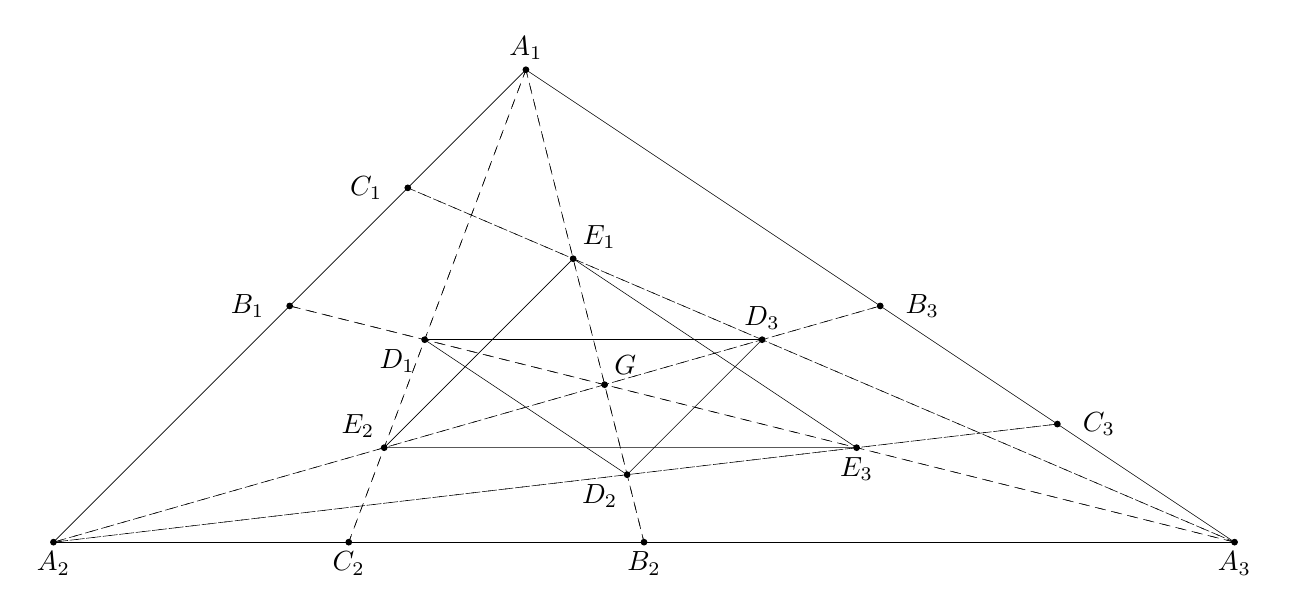
\begin{tikzpicture}[scale=3]
			% \useasboundingbox (-2,-2) rectangle  (2,2);
			\tkzDefPoint(0,2){A_1}
			\tkzDefPoint(-2,0){A_2}
			\tkzDefPoint(3,0){A_3}
			\tkzDefBarycentricPoint(A_1=1,A_2=1,A_3=1)\tkzGetPoint{G}
			\tkzDefBarycentricPoint(A_1=1,A_2=1)\tkzGetPoint{B_1}
			\tkzDefBarycentricPoint(A_2=1,A_3=1)\tkzGetPoint{B_2}
			\tkzDefBarycentricPoint(A_3=1,A_1=1)\tkzGetPoint{B_3}
			\tkzDefBarycentricPoint(A_1=1,B_1=1)\tkzGetPoint{C_1}
			\tkzDefBarycentricPoint(A_2=1,B_2=1)\tkzGetPoint{C_2}
			\tkzDefBarycentricPoint(A_3=1,B_3=1)\tkzGetPoint{C_3}
			\tkzInterLL(A_1,C_2)(B_1,A_3)\tkzGetPoint{D_1}
			\tkzInterLL(A_2,C_3)(B_2,A_1)\tkzGetPoint{D_2}
			\tkzInterLL(A_3,C_1)(B_3,A_2)\tkzGetPoint{D_3}
			\tkzInterLL(A_1,B_2)(C_1,A_3)\tkzGetPoint{E_1}
			\tkzInterLL(A_2,B_3)(C_2,A_1)\tkzGetPoint{E_2}
			\tkzInterLL(A_3,B_1)(C_3,A_2)\tkzGetPoint{E_3}
			\tkzDrawSegments(A_1,A_2 A_2,A_3 A_3,A_1)
			\tkzDrawSegments[dashed](A_1,C_2 A_2,C_3 A_3,C_1 A_1,B_2 A_2,B_3 A_3,B_1)
			\tkzDrawSegments[dashed](B_1,A_3 B_2,A_1 B_3,A_2 C_1,A_3 C_2,A_1 C_3,A_2)
			\tkzDrawSegments(D_1,D_2 D_2,D_3 D_3,D_1)
			\tkzDrawSegments(E_1,E_2 E_2,E_3 E_3,E_1)
			\tkzDrawPoints[fill=black](A_1,A_2,A_3,B_1,B_2,B_3,C_1,C_2,C_3,D_1,D_2,D_3,E_1,E_2,E_3,G)
			\tkzLabelPoints[above](A_1,D_3)
			\tkzLabelPoints[right=0.2](B_3,C_3)
			\tkzLabelPoints[below](A_2,A_3,B_2,C_2,E_3)
			\tkzLabelPoints[left=0.2](B_1,C_1)
			\tkzLabelPoints[above left](E_2)
			\tkzLabelPoints[above right](E_1,G)
			\tkzLabelPoints[below left](D_2,D_1)
			\end{tikzpicture}
		\end{center}		
		\end{figure}
	We use Menelause's \thm\ on the following sets of points $\left\{\{A_1 E_2 C_2\},\{A_2 E_3 C_3\},\{A_3 E_1 C_1\}\right\}$ to get that
	\begin{flalign}
		&&\frac{GE_1}{E_1 A_1}&=\frac{GE_2}{E_2 A_2}=\frac{GE_3}{E_3 A_3}=\frac{2}{3}&\nonumber\\
		&\Rightarrow&\frac{GE_1}{GA_1}&=\frac{GE_2}{GA_2}=\frac{GE_3}{GA_3}=\frac{2}{5}&\nonumber\\
		&\Rightarrow&\frac{|\triangle E_1 E_2 E_3|}{|\triangle A_1 A_2 A_3|}&=\left( \frac{2}{5} \right)^{2}=\frac{4}{25} &\nonumber
	\end{flalign}
	We then use Menelause's \thm\ on the sets of points $\left\{\{A_1 D_2 B_2\},\{A_2 D_3 B_3\},\{A_3 D_1 B_1\}\right\}$ and then on the sets of points $\left\{\{A_1 G C_2\},\{A_2 G C_3\},\{A_3 G C_1\}\right\}$ to get that
	\begin{flalign}
		&&\frac{D_1 C_2}{A_1 D_1}&=\frac{D_2 C_3}{A_2 D_2}=\frac{D_3 C_1}{A_3 D_3}=\frac{3}{4}&\nonumber\\
		&\Rightarrow&\frac{A_1 C_2}{A_1 D_1}&=\frac{A_2 C_3}{A_2 D_2}=\frac{A_3 C_1}{A_3 D_3}=\frac{7}{4}&\nonumber\\
		&\Rightarrow&\frac{D_1 G}{G A_3}&=\frac{D_2 G}{G A_1}=\frac{D_3 G}{G A_2}=\frac{2}{7}&\nonumber\\
		&\Rightarrow&\frac{|\triangle D_1 D_2 D_3|}{|\triangle A_1 A_2 A_3|}&=\left( \frac{2}{7} \right)^{2}=\frac{4}{49} &\nonumber\\
		&\Rightarrow&\frac{|\triangle D_1 D_2 D_3|}{|\triangle E_1 E_2 E_3|}&=\frac{25}{49} &\nonumber
	\end{flalign}
	\end{proof}

	
	
\end{document}